% !TEX root = ../main.tex
\section{Detailed Illustrative Examples}
\label{app:detailed-examples}

\subsection{Additive Noise: Exact Trajectories and Horizon Tuning}
\label{app:additive-details}

For explicit constants, specialize the additive example to
\begin{equation}
\label{eq:additive-comparison-oracle}
f(x)=\frac{x^2}{2},\qquad h(x,\xi)=x+\xi,\qquad
\mathbb P(\xi=1)=\mathbb P(\xi=-1)=\frac12,\qquad x_0=1.
\end{equation}
Here $L=1$, $\Delta_0=1/2$, $\sigma^2=1$, and $\delta=0$.
At $\eta=1$, SGD satisfies $x_{k+1}=-\xi_k$, hence
\begin{equation}
\label{eq:additive-sgd-fixed}
G_k^{\mathrm{SGD}}=1\quad(k\geq0),\qquad
\boxed{\overline G_K^{\mathrm{SGD}}=1.}
\end{equation}
Thus the fixed-step noise floor is present in the actual trajectory.

For the horizon-dependent BV stepsize
\eqref{eq:sgd-bv-optimal-step}, write
$\eta_K=2/(1+\sqrt{1+4K})$ and $r_K=1-\eta_K$.
Independence and centeredness of the fresh sample give
\[
G_{k+1}^{\mathrm{SGD}}
=\mathbb E[(r_Kx_k-\eta_K\xi_k)^2]
=r_K^2G_k^{\mathrm{SGD}}+\eta_K^2.
\]
Solving from $G_0=1$ and averaging the geometric terms yields
\begin{align*}
G_k^{\mathrm{SGD}}
&=r_K^{2k}+\frac{\eta_K}{2-\eta_K}(1-r_K^{2k}),\\
\overline G_K^{\mathrm{SGD}}
&=\frac{\eta_K}{2-\eta_K}
+\left(1-\frac{\eta_K}{2-\eta_K}\right)
\frac{1-r_K^{2K}}{K(1-r_K^2)}.
\end{align*}
Since $\eta_K\sim K^{-1/2}$,
$r_K^{2K}\leq e^{-2K\eta_K}\to0$ and
$1-r_K^2=\eta_K(2-\eta_K)\sim2K^{-1/2}$.
Each term in the average is therefore asymptotic to $1/(2\sqrt K)$:
\begin{equation}
\label{eq:additive-sgd-tuned}
\boxed{\overline G_K^{\mathrm{SGD}}=\frac{1+o(1)}{\sqrt K}.}
\end{equation}
The optimized BV bound is $(1+\sqrt{1+4K})/(2K)$, so both its
rate and leading constant are attained by this prescribed run.

For TSGD, use $\eta=1$ and any square-integrable $g_0=1+e_0$.
Exact differences give $D_{k+1}=x_{k+1}-x_k=-g_k$;
therefore $g_1=0$ and $x_k=-e_0$ for all $k\geq1$. Hence
\begin{equation}
\label{eq:additive-tsgd-exact}
\boxed{\overline G_K^{\mathrm{TSGD}}
=\frac1K+\left(1-\frac1K\right)E_0.}
\end{equation}
With exact initialization, TSGD reaches the minimizer after one
step. For fixed $E_0>0$, horizon-tuned SGD eventually has the smaller
error. The comparison depends on initialization as well as transport.

\subsection{Multiplicative Noise: Fresh Gradients and False Convergence}
\label{app:multiplicative-details}

For \eqref{eq:multiplicative-comparison-oracle},
$\mathbb E[a]=1$ and $\mathbb E[(a-1)^2]=1$. The oracle is
unbiased and its pointwise noise variance is $x^2$, so global BV
does not hold. Coupled centered differences nevertheless satisfy
\[
\mathbb E[|(a-1)(x-y)|^2]=|x-y|^2,
\]
giving $\delta=1$. These comparisons use exact dynamics rather
than the BV theorem.

At $\eta=1/2$, SGD obeys $x_{k+1}=(1-a_k/2)x_k$;
it remains at one until the first sample $a=2$, then stays at zero.
Thus
\begin{equation}
\label{eq:multiplicative-sgd-exact}
\boxed{G_k^{\mathrm{SGD}}=2^{-k},\qquad
\overline G_K^{\mathrm{SGD}}=\frac{2(1-2^{-K})}{K}.}
\end{equation}
For TSGD at the same step, let $g_0=\nabla f(x_0)=1$ and
$N:=\min\{n\geq1:a_n=2\}$. The estimator recursion is
$g_{k+1}=(1-a_{k+1}/2)g_k$, so
\[
\mathbb P(N=n)=2^{-n},\qquad
g_k=\boldsymbol 1_{\{k<N\}},\qquad
x_k=1-\frac12\min\{k,N\}.
\]
Since $N<\infty$ almost surely and $\mathbb E[N^2]=6$,
dominated convergence gives $x_k\to1-N/2$ in mean square.
Using $\mathbb E[N]=2$,
\begin{equation}
\label{eq:multiplicative-tsgd-residual}
\boxed{\lim_{k\to\infty}G_k^{\mathrm{TSGD}}
=\mathbb E[(1-N/2)^2]=\frac12.}
\end{equation}
The estimator becomes zero almost surely in finite time, but the
limiting true gradient is nonzero with probability
$1-\mathbb P(N=2)=3/4$. Ces\`aro averaging also gives
$\overline G_K^{\mathrm{TSGD}}\to1/2$.

\subsection{Sharpness for Horizon-Tuned TSGD}
\label{app:proof-multiplicative-tsgd-tuned}

For the same oracle with exact initialization,
\eqref{eq:tsgd-optimal-step} gives
$\eta_K^\star=2/(1+\sqrt{4K-3})$, since
$L=\delta=1$ and $\Delta_0=1/2$.
The optimized guarantee becomes
\begin{equation}
\label{eq:multiplicative-tsgd-tuned-bound}
\overline G_K^{\mathrm{TSGD}}
\leq\frac{1+\sqrt{4K-3}}{2K}.
\end{equation}

\begin{lemma}[Asymptotic sharpness for tuned TSGD]
\label{lem:multiplicative-tsgd-tuned-exact}
For \eqref{eq:multiplicative-comparison-oracle}, with exact
initialization and the constant step $\eta_K^\star$ for the
$K$-iteration run,
\[
\lim_{K\to\infty}\sqrt K\,\overline G_K^{\mathrm{TSGD}}=1.
\]
\end{lemma}

\begin{proof}
Fix $K\geq2$ and write $\eta=\eta_K^\star$. The updates imply
\[
g_{k+1}=(1-\eta a_{k+1})g_k,\qquad
e_{k+1}=e_k+\eta(1-a_{k+1})g_k.
\]
Set $C_k:=\mathbb E[g_ke_k]$ and
$q:=\mathbb E[(1-\eta a)^2]=1-2\eta+2\eta^2$.
Independence yields
\[
M_{k+1}=qM_k,\qquad E_{k+1}=E_k+\eta^2M_k,
\qquad C_{k+1}=(1-\eta)C_k+\eta^2M_k.
\]
Starting from $M_0=1$ and $E_0=C_0=0$, these give
\[
M_k=q^k,\qquad E_k=\frac{\eta}{2(1-\eta)}(1-q^k),\qquad
C_k=\eta^2\sum_{t=0}^{k-1}(1-\eta)^{k-1-t}q^t.
\]
Since $0<\eta<1$ and $q<1$, all summands are nonnegative and
\[
\sum_{k<K}C_k
\leq\eta^2\left(\sum_{t\geq0}q^t\right)
             \left(\sum_{j\geq0}(1-\eta)^j\right)
=\frac{\eta^2}{(1-q)\eta}
=\frac1{2(1-\eta)}.
\]
Thus the average cross moment is $O(K^{-1})$ as
$\eta_K^\star\to0$. For the other moments,
\[
\frac1K\sum_{k<K}M_k=\frac{1-q^K}{K(1-q)},\qquad
\frac1K\sum_{k<K}E_k=
\frac{\eta}{2(1-\eta)}
\left(1-\frac1K\sum_{k<K}M_k\right).
\]
Now $\eta_K^\star\sim K^{-1/2}$,
$1-q=2\eta_K^\star(1-\eta_K^\star)\sim2K^{-1/2}$, and
$q^K\leq e^{-K(1-q)}\to0$. Therefore
\[
\frac1K\sum_{k<K}M_k\sim\frac1{2\sqrt K},\qquad
\frac1K\sum_{k<K}E_k\sim\frac1{2\sqrt K}.
\]
Finally, $x_k=g_k-e_k$ implies
$G_k=M_k+E_k-2C_k$. The averaged cross term is lower order,
which proves the claim.
\end{proof}

The theorem's bound has the correct leading rate and constant for
this prescribed TSGD run. Fixed-step SGD in
\eqref{eq:multiplicative-sgd-exact} has average error
$\Theta(K^{-1})$, whereas this horizon-tuned TSGD run has
$\Theta(K^{-1/2})$ error. This is not a lower bound over all TSGD
stepsize schedules.

\subsection{Fixed Variance and Variable Similarity}
\label{app:sinusoidal-proof}

\begin{lemma}[Fixed variance and variable similarity]
\label{lem:fixed-variance-variable-similarity}
For \eqref{eq:fixed-variance-oracle}, the noise is centered, satisfies
\eqref{eq:phase-noise-moments}, and has smallest global similarity
constant $\delta=\sigma\omega$ for $\omega\geq0$.
\end{lemma}

\begin{proof}
A uniform phase makes the cosine have mean zero and second moment
$1/2$, so
$\mathbb E[r(x,\varphi)^2]=2\sigma^2(1/2)=\sigma^2$.
For the coupled difference,
\[
r(x,\varphi)-r(y,\varphi)
=-2\sqrt2\sigma
\sin\!\left(\frac{\omega(x+y)}2+\varphi\right)
\sin\!\left(\frac{\omega(x-y)}2\right).
\]
Squaring and using
$\mathbb E_\varphi[\sin^2(c+\varphi)]=1/2$ for every fixed $c$ gives
\[
\mathbb E[|r(x,\varphi)-r(y,\varphi)|^2]
=8\sigma^2\cdot\frac12\,
  \sin^2\!\left(\frac{\omega(x-y)}2\right)
=4\sigma^2\sin^2\!\left(\frac{\omega(x-y)}2\right).
\]
This verifies \eqref{eq:phase-noise-moments}.
The inequality $|\sin t|\leq|t|$ proves similarity with
$\delta=\sigma\omega$; minimality follows from
\[
\lim_{y\to x}
\frac{4\sigma^2\sin^2(\omega(x-y)/2)}{(x-y)^2}
=\sigma^2\omega^2.
\]
\end{proof}

SGD's fresh noise has conditional variance $\sigma^2$ at every
iterate, giving the frequency-independent exact recursion
\begin{equation}
\label{eq:phase-sgd-dynamics}
G_{k+1}^{\mathrm{SGD}}
=(1-L\eta)^2G_k^{\mathrm{SGD}}+L^2\eta^2\sigma^2.
\end{equation}
Indeed, even its conditional noise distribution is independent of
$x_k$ and $\omega$, since adding $\omega x_k$ to a uniform phase
preserves its distribution modulo $2\pi$. For TSGD,
\begin{equation}
\label{eq:phase-tsgd-error}
\begin{aligned}
E_{k+1}-E_k
&=4\sigma^2\mathbb E\!\left[
\sin^2\!\left(\frac{\omega(x_{k+1}-x_k)}2\right)\right]\\
&\leq\sigma^2\omega^2\eta^2M_k.
\end{aligned}
\end{equation}
For fixed $\sigma>0$, varying $\omega$ realizes any smallest global
similarity constant without changing the pointwise noise distribution.
The sine factor also shows that
increasing $\omega$ need not increase every realized increment's
error monotonically.

\subsection{Least-Squares Experiments}
\label{app:ls}

We use one least-squares model to illustrate initialization quality,
label-noise cancellation, false convergence, and the effect of similarity.
The figures compare iterations at a common stepsize, not computational
cost or optimally tuned performance.

\paragraph{Common setup.}
Let $f(x)=\tfrac12\mathbb E[\|Ax-b\|^2]$, with
\[
H=\operatorname{diag}(0.1,0.2,\ldots,1),\qquad
A=\sqrt v\,H^{1/2},\qquad b=s\varepsilon,
\]
where $v=1+\kappa\zeta$, $\mathbb P(\zeta=1)=\mathbb P(\zeta=-1)=1/2$,
and $\varepsilon\sim\mathcal N(0,I_{10})$ is independent of $\zeta$.
The minimizer is $x^\star=0$, and
\[
\nabla f(x)=Hx,\qquad
h(x;v,\varepsilon)=vHx-s\sqrt v\,H^{1/2}\varepsilon,\qquad
h(x;v,\varepsilon)-h(y;v,\varepsilon)=vH(x-y).
\]
Thus label noise, controlled by $s$, cancels from shared-sample
differences, while feature variability determines $\delta=\kappa$.
We use $x_0=\boldsymbol 1/\|H\boldsymbol 1\|$,
$\eta=0.5$, and 4,000 independent trajectories.
The figures show the first 80 of 400 updates, with pointwise bands
of $\pm2$ Monte Carlo standard errors.
Initial estimates are independent of subsequent samples.

\paragraph{Initialization quality.}
In Figure~\ref{fig:ls-init}, $s=1$ and $\kappa=0.05$:
gradients are noisy but their differences are accurate.
TSGD initializes by averaging $B_0\in\{1,128,512\}$ actual stochastic
gradients; SGD uses one fresh sample at every update.
Single-sample initialization leaves TSGD with a larger residual than
SGD, whereas the larger initial batches give smaller residuals.
Accurate transport preserves useful initial information but does not
correct a poor initial estimate. The extra cost of larger initial
batches is not reflected in the iteration axis.

\paragraph{False convergence.}
Figure~\ref{fig:ls-main}(b) uses noiseless labels ($s=0$),
$\kappa=0.9$, and $B_0=128$ sampled gradients to initialize TSGD.
SGD's true gradient and TSGD's estimator both tend to zero in mean
square, but TSGD's true-gradient error remains positive.
The plot therefore distinguishes a small estimator from actual
stationarity.

\paragraph{Label-noise cancellation.}
In Figure~\ref{fig:ls-main}(a), both methods instead start from the
exact gradient. We fix $\kappa=0.2$ and use matched feature draws
across $s\in\{0,1,5\}$. TSGD's trajectories coincide because label noise
cancels from every difference; its remaining error comes from feature
variability. SGD's residual grows with label noise and vanishes at $s=0$.

\paragraph{Initialization and similarity.}
\label{app:quad-numerics}
Figure~\ref{fig:ls-errors} prescribes
$g_0=Hx_0+e_0$, with $e_0\sim\mathcal N(0,(E_0/10)I_{10})$,
independently of subsequent samples. We vary
$\delta=\kappa\in\{0.05,0.9\}$ and $E_0\in\{10^{-3},10^{-1}\}$.
Applying \eqref{eq:quadratic-interaction} coordinatewise gives
\begin{equation}
\label{eq:least-squares-residual}
\lim_kG_k=E_0+\sum_{j=1}^{10}
\frac{\eta\kappa^2\lambda_j}
 {2-\eta(1+\kappa^2)\lambda_j}
\left(\lambda_j^2x_{0,j}^2+\frac{E_0}{10}\right).
\end{equation}
The denominators are positive for our parameters.
The plateaus agree with these limits: better initialization reduces both
inherited and transport error, while smaller $\delta$ reduces the
transport contribution. This experiment and the label-noise experiment
use controlled estimates, unlike the sampled initialization in the
other two; they do not model how the initial accuracy is obtained.

\begin{figure}[t]
\centering
\begin{minipage}{0.49\linewidth}
\centering
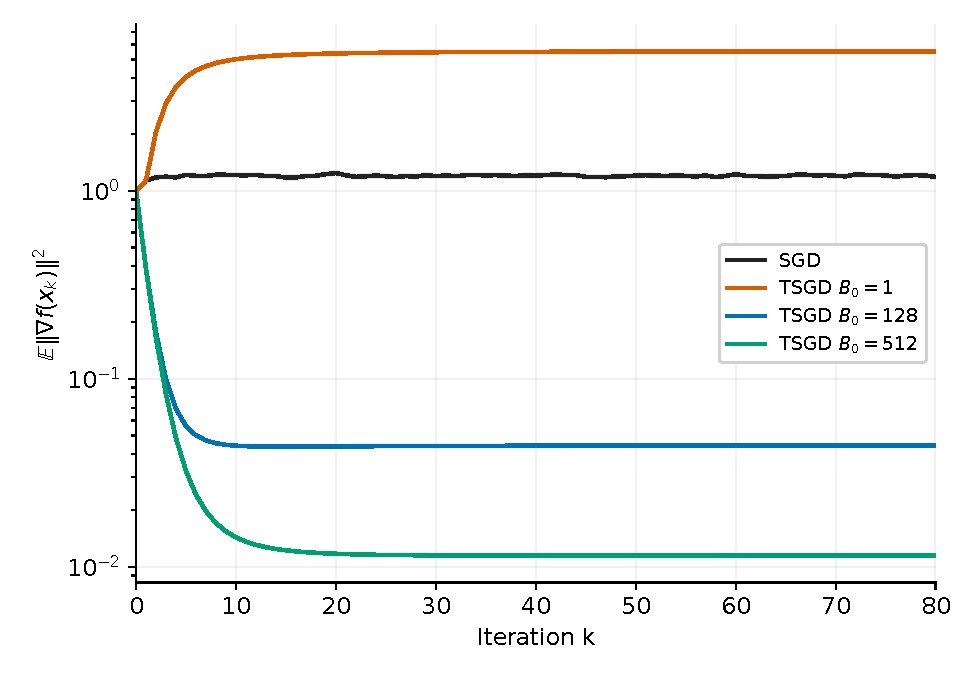
\includegraphics[width=\linewidth]{figures/least_squares_A.pdf}
\caption{Sampled initialization: increasing $B_0$ lowers the residual
when differences are accurate.}
\label{fig:ls-init}
\end{minipage}\hfill
\begin{minipage}{0.49\linewidth}
\centering
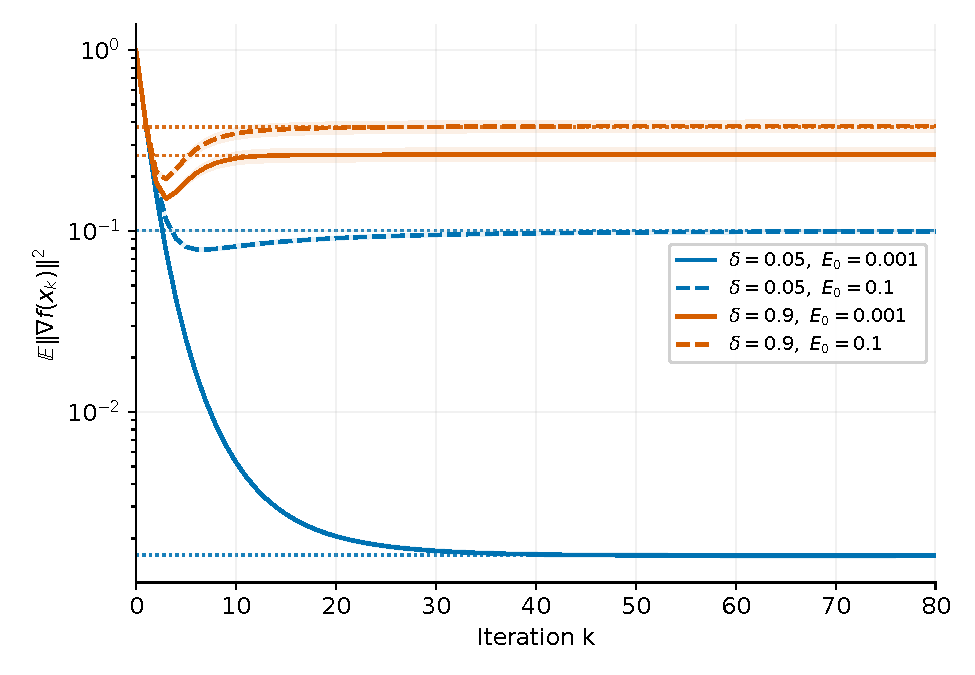
\includegraphics[width=\linewidth]{figures/least_squares_D.pdf}
\caption{Controlled initialization: varying $E_0$ and $\delta$.
Dotted lines give the exact limits in
\eqref{eq:least-squares-residual}.}
\label{fig:ls-errors}
\end{minipage}
\end{figure}
